% !TEX root = ../main.tex




\item\pt{5}\begin{minipage}[t]{.7\textwidth}
(\emph{Toestel van Atwood}) Twee verschillende massa's zijn via een katrol van te verwaarlozen massa met elkaar verbonden zoals in de figuur. De wrijving is eveneens te verwaarlozen. 
\newline
\newline
Bepaal de grootte van de versnelling van beide massa's en de spankracht in het touw.
\end{minipage}
\hfill
\begin{minipage}[t]{.2\textwidth}
\flushright
	\raisebox{1ex-\height}{%
		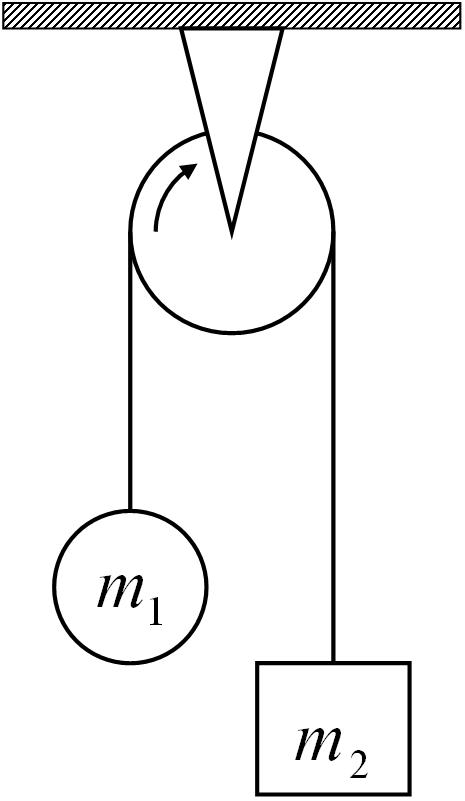
\includegraphics[height=4cm]{toestelatwood}
	}
\end{minipage}

\begin{oplossing}
$a=\frac{m_2-m_1}{m_1+m_2}g \quad F_s=\frac{2m_1m_2}{m_1+m_2}g$
\end{oplossing}